% =====================================================================
% Modelo para Subprojeto de Iniciação Científica (em Português)
% Prof. Vítor E. Silva Souza - NEMO/UFES :: DI/UFES :: PPGI/UFES
%
% Baseado no modelo fornecido pela PRPPG/UFES:
% https://prppg.ufes.br/programa-institucional-de-ic-piic
% =====================================================================
\documentclass[10pt, a4paper]{article}

\usepackage[pdftex]{graphicx,color}
\usepackage[dvipsnames]{xcolor,colortbl}
\usepackage[hidelinks]{hyperref}
\usepackage{anysize}
\usepackage{graphicx}
\usepackage[utf8]{inputenc}
\usepackage[portuges,brazilian]{babel}
\usepackage{fancyhdr}
\usepackage{ifthen}
\usepackage{array}
\usepackage{natbib}
%\usepackage{ tipa }
\usepackage{amssymb}
\usepackage{amsmath}
%\usepackage[usenames,dvipsnames]{xcolor} %to allow for color changes
%\definecolor{light-gray}{gray}{0.80} % defines the colour.
%\usepackage{cite} % to allow line breaks inside citations

%% Para redução de espaço entre os itens da bibliografia
	\let\oldbibliography\thebibliography
	\renewcommand{\thebibliography}[1]{\oldbibliography{#1}
	\setlength{\itemsep}{0pt}}

\usepackage{helvet}
\renewcommand{\familydefault}{\rmdefault}

\usepackage{enumerate}
\usepackage{adjustbox}

\usepackage{parskip}% http://ctan.org/pkg/parskip
\setlength{\parindent}{0pt}

\linespread{1.25}

\usepackage{titlesec}

\titleformat{\section}
  {\normalfont\Large\bfseries}{\thesection}{1em}{}[{\titlerule[0.8pt]}]

\newcommand{\mnras}{Mon. Not. R. Astron. Soc.}
\newcommand{\aap}{Astronomy $\&$ Astrophysics}
\newcommand{\apjs}{ApJS}
\newcommand{\apj}{Astrophys. J.}
\newcommand{\apjl}{Astrophys. J. Letters}
\newcommand{\aj}{Astron. J.}
\newcommand{\pasa}{PASA}
\newcommand{\nat}{Nature}

\usepackage{mathptmx}
\usepackage{tabularx}

\usepackage{caption}
\usepackage{subcaption}

\usepackage{newfloat}
\DeclareFloatingEnvironment[name={Gráfico}]{grafico}
\DeclareFloatingEnvironment[name={Quadro}]{quadro}

\usepackage{enumitem}
\setlist[enumerate]{nosep}

% Colorinlistoftodos package: to insert colored comments so authors can collaborate on the content.
\usepackage[colorinlistoftodos, textwidth=20mm, textsize=footnotesize]{todonotes}
\newcommand{\aluno}[1]{\todo[author=\textbf{Aluno},color=green!30,caption={},inline]{#1}}
\newcommand{\professor}[1]{\todo[author=\textbf{Professor},color=red!30,caption={},inline]{#1}}

% Permite usar o comando \hl{} para evidenciar texto com fundo amarelo. Útil para chamar atenção a itens a fazer.
\usepackage{soulutf8}

%\marginsize{left}{right}{top}{bottom}
\marginsize{30mm}{20mm}{30mm}{20mm}

%\renewcommand{\arraystretch}{1.5}


\usepackage{fancyhdr}
\usepackage{afterpage}
\pagestyle{fancy}
\fancyhf{} % clear all fields
\fancyhead[R]{\color{Gray} Universidade Federal do Espírito Santo\\ Programa Institucional de Iniciação Científica\\ Relatório Final de Pesquisa\\ {\color{Red} Grande Área do Conhecimento (CNPq)}}
\setlength{\headheight}{40pt}
\renewcommand{\headrulewidth}{0pt}

%\pagenumbering{arabic}

% Pacote xspace: para colocar espaços no final das macros quando necessário.
\usepackage{xspace}


% Definição de macros.
\newcommand{\java}{Java\texttrademark\xspace}



\begin{document}

\afterpage{\cfoot{\thepage}}



\begin{center}
 {\Large \bf  {\color{Red} Título do Subprojeto de Iniciação Científica -- PIIC/UFES}}
 \end{center}

\vspace{.5cm}


\bgroup
\def\arraystretch{1.3}
\begin{tabularx}{\textwidth}{|>{\columncolor{gray!25}}l|X|}
\hline
{\bf Edital:} & Edital PIIC 20\_\_ /20\_\_ \\
\hline
{\bf Grande Área do Conhecimento (CNPq):} &  \\
\hline
{\bf Área do Conhecimento (CNPq):} &  \\
\hline
{\bf Título do Projeto:} &  \\
\hline
{\bf Título do Subprojeto:} &  \\
\hline
{\bf Professor(a) Orientador(a):}&   \\
\hline
{\bf Estudante:} &   \\
\hline
\end{tabularx}
\egroup

\vspace{.5cm}

%\bigskip


%%%%%%%%%%%%%%%%%%%%%%%%%%%%%
\section*{Resumo}

A NBR 6028:2003 estabelece os requisitos para redação e apresentação de resumos, definindo-os como sendo uma ``apresentação concisa dos pontos relevantes de um documento''~\citep[p. 1]{abnt:nbr6028}. No caso do Relatório Final de Pesquisa, este resumo seria do tipo informativo, isto é, que deve informar ao leitor uma breve contextualização do tema do trabalho realizado, as justificativas, os objetivos, a metodologia adotada, os resultados obtidos, e as conclusões. O texto do resumo deve ser composto de uma sequência de frases concisas, afirmativas (e não de enumeração de tópicos), em um parágrafo único. Por outro lado, devem-se evitar citações, símbolos e contrações que não sejam de uso corrente, bem como fórmulas, equações, diagramas e etc. Quanto à sua extensão, o Resumo deve ter de 150 a 200 palavras.
      
{\bf Palavras-chave:} As palavras-chave devem figurar logo abaixo do resumo, antecedidas da expressão ``Palavras-chave:'', separadas entre si por ponto e finalizadas também por ponto. Devem fornecer ao leitor uma ideia dos principais temas de interesse de que trata a pesquisa. Podem ser informadas, no máximo, 06 (seis) palavras chave.
      

  
%%%%%%%%%%%%%%%%%%%%%%%%%%%%%
\section{Introdução}
\label{sec-intro}

Este documento deve ser utilizado como modelo para a elaboração do Relatório Final de Pesquisa no âmbito do Programa Institucional de Iniciação Científica (PIIC) da UFES. Deve ser composto das seguintes seções: resumo, introdução, objetivos, referencial teórico, metodologia, resultados, conclusões e referências bibliográficas. 

O texto do Relatório Final de Pesquisa deve ser preparado considerando que todas as seções que compõem o documento não excedam 15 páginas de formato A4 com margens de 3 cm (esquerda e superior) e de 2 cm (direita e inferior), usando fonte Times New Roman, tamanho da fonte 10, com espaçamento entre linhas de 1,5, sem recuo na primeira linha de cada parágrafo e com alinhamento justificado. Já os títulos das seções também devem utilizar a fonte Times New Roman, mas com tamanho 12. Por fim, o cabeçalho de todas as páginas deve ser mantido de acordo com a formatação deste modelo (Times New Roman, tamanho 9, alinhado à direita), sendo que a quarta linha do cabeçalho deve ser alterada para a cor preto e descrever a Grande Área do Conhecimento do projeto segundo o Conselho Nacional de Desenvolvimento Científico e Tecnológico (CNPq), isto é, Ciências Exatas e da Terra, Ciências Biológicas, Engenharias, Ciências da Saúde, Ciências Agrárias, Ciências Sociais Aplicadas, Ciências Humanas ou Linguística, Letras e Artes. O título do Subprojeto de Iniciação Científica deve ser inserido no lugar de ``Título do Subprojeto de Iniciação Científica – PIIC/UFES'' e sua cor, também trocada para preto.

Por outro lado, a linguagem utilizada ao longo do trabalho deve ser técnica e impessoal, afinal, trata-se de um trabalho acadêmico. Deve-se evitar o uso de gírias e de termos de linguagem coloquial, bem como o uso de concordâncias nas primeiras pessoas do singular e do plural (fiz ou fizemos...; obtive ou obtivemos...). Nestes casos, deve-se utilizar da impessoalidade por meio do uso da terceira pessoa (fez-se...; foram obtidos...). 

O conteúdo de cada seção deve estar de acordo com as recomendações descritas neste modelo. Na Introdução, o autor deve apresentar uma contextualização do tema de sua pesquisa, mostrando sua relevância, justificando o tema escolhido, e descrevendo claramente a sua pergunta de pesquisa ou problema de pesquisa, citando, sempre que possível, trabalhos de outros autores. Nesta seção, deve-se também ressaltar a ligação do Subprojeto de Iniciação Científica com o Projeto de Pesquisa ao qual está vinculado.



%%%%%%%%%%%%%%%%%%%%%%%%%%%%%
\section{Objetivos}
\label{sec-objetivos}

A seção Objetivos deve conter, de forma concisa, quais foram os objetivos geral e específicos do Subprojeto de Iniciação Científica, ou seja, as hipóteses que se quis demonstrar, os dispositivos que se quis montar, os compostos que se desejava sintetizar, as ideias que se desejava corroborar ou refutar e etc. Também deve apresentar, de forma concisa, as razões pelas quais se desejava atingir estes objetivos.



%%%%%%%%%%%%%%%%%%%%%%%%%%%%%
\section{Embasamento Teórico}
\label{sec-embasamento}

De acordo com \cite{prodanov-freitas:book2013} ``Embasamento Teórico'' compreende ``elementos de fundamentação teórica da pesquisa e, também, a definição dos conceitos empregados'' à realização do trabalho. Os elementos de fundamentação teórica da pesquisa, a revisão da bibliografia e a definição dos termos e conceitos aplicados na pesquisa devem ser aqui reportados.

Normalmente, há várias citações nesta seção, que são trechos transcritos ou informações retiradas de outras fontes (escrita ou oral), inseridos no texto com o propósito de esclarecer, complementar e até mesmo sustentar as ideias do autor do trabalho. Como se tratam de informações de autoria diferente do trabalho acadêmico em questão, a fonte de onde foi extraída deve ser obrigatoriamente identificada para fins de garantia e respeito dos direitos autorais. Todas as obras citadas no texto devem fazer parte da lista de referências na seção ``Referências Bibliográficas'', seguindo as regras de apresentação definidas na ABNT NBR 6023:2018.

As citações podem acontecer de três formas distintas ao longo do trabalho:
\begin{enumerate}[label=\alph*)]
\item \textbf{Citação direta} –- quando é feita a transcrição literal de textos de outros autores. Ou seja, utilizam-se as mesmas palavras do autor consultado no texto que está sendo escrito;

\item \textbf{Citação indireta} –- quando ocorre apenas a reprodução da ideia sem a transcrição literal do texto do autor consultado. Neste caso, as palavras utilizadas no texto que está sendo escrito são diferentes das adotadas pelo autor consultado, mas a ideia (informação) transmitida é a mesma;

\item \textbf{Citação de citação} –- nos casos em que não for possível consultar o documento original, pode-se fazer a transcrição (direta ou indireta) de uma informação já citada por outros autores. No entanto, todo esforço deve ser empreendido para que a fonte original da informação seja consultada antes de se utilizar desse tipo de citação.
\end{enumerate}

Neste Relatório Final de Pesquisa, a identificação das citações deve ser incluída no texto e a chamada das mesmas deve utilizar o sistema autor-data, tudo conforme a ABNT NBR 10520:2002~\citep{abnt:nbr10520}.




%%%%%%%%%%%%%%%%%%%%%%%%%%%%%
\section{Metodologia}
\label{sec-metodo}

A metodologia que foi adotada para testar a hipótese formulada e atingir os objetivos estabelecidos deve ser aqui detalhada, classificando a pesquisa realizada do ponto de vista da sua natureza, dos seus objetivos, dos procedimentos técnicos e da forma de abordagem do problema de pesquisa. Necessita ainda apresentar os procedimentos de trabalho, os materiais que foram utilizados, o tratamento da informação realizado e o procedimento estatístico aplicado, se for o caso. Esta seção deve, entretanto, além de detalhar os aspectos da metodologia empregada nas atividades especificamente executadas pelo estudante, apresentar sua relação com o Projeto de Pesquisa ao qual o Subprojeto de Iniciação Científica está vinculado.




%%%%%%%%%%%%%%%%%%%%%%%%%%%%%
\section{Resultados e Discussão}
\label{sec-resultados}

Esta seção deve explicitar os resultados ou respostas encontradas durante o trabalho de pesquisa, apresentando os dados/informações obtidos(as) ou coletados(as) e incluindo ilustrações, figuras, fotos ou esquemas.

Além de expor os resultados encontrados, os mesmos devem ser interpretados, analisados e relacionados com o ``Embasamento Teórico'' existente e abordado anteriormente na seção 3. Ou seja, deve haver uma discussão sobre o significado dos resultados obtidos, contemplando, preferencialmente, os seguintes aspectos: 

\begin{itemize}
	\item O que estas respostas ou dados obtidos significam? 
	\item Como elas ajudam a resolver o problema? 
	\item Descrição dos dados à luz da literatura, isto é, como as respostas obtidas se comparam com os dados de literatura.
	\item Quais as possíveis fontes de erro e seu efeito sobre os dados ou análises?
\end{itemize}

Quanto às ilustrações (figuras, gráficos, fluxogramas, quadros e etc.) e tabelas, estas devem ser utilizadas a fim de explicar ou complementar visualmente o texto. Desta forma, torna-se obrigatória a inclusão de um comentário sobre a ilustração ou a tabela no texto. A NBR 15287:2011 reforça este fato quando diz que ``A ilustração deve ser citada no texto e inserida o mais próximo possível do trecho a que se refere.''~\citep[p. 8]{abnt:nbr15287}. Cabe ressaltar que a citação no texto sempre deve preceder a ilustração ou a tabela. Estes elementos devem estar centralizados na página, sua identificação na parte superior e a indicação da fonte consultada (elemento obrigatório, mesmo que seja produção do próprio autor), legenda, notas e outras informações necessárias à sua compreensão (se houver), na parte inferior (alinhados à borda esquerda da ilustração e limitados pela borda direita da mesma), como mostra a Figura~\ref{fig-exemplo} e o Gráfico~\ref{graf-exemplo}.

\begin{figure}[h!]
	\centering
	\caption{(a) Fotografia do modelo de edificação utilizado no experimento e (b) representação esquemática do comportamento do escoamento sobre a edificação}
	\label{fig-exemplo}
	\begin{subfigure}[b]{0.45\textwidth}
		\centering
		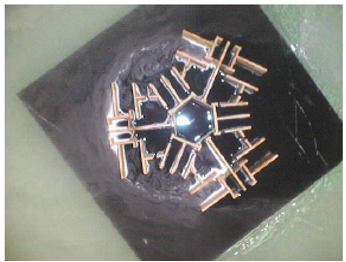
\includegraphics[width=\textwidth]{fig-exemploA}
		\caption{}
		\label{fig-exemploA}
	\end{subfigure}
	\hfill
	\begin{subfigure}[b]{0.45\textwidth}
		\centering
		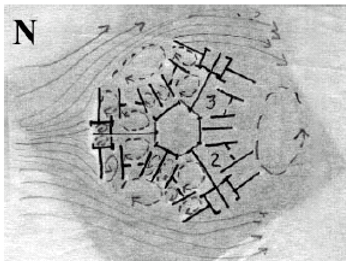
\includegraphics[width=\textwidth]{fig-exemploB}
		\caption{}
		\label{fig-exemploB}
	\end{subfigure}
	\caption*{Fonte: \cite{toledo-pereira:clacs2004}.}
\end{figure}

\begin{grafico}[h!]
	\centering
	\caption{Consumo final de energia por fonte no Brasil em 2011}
	\label{graf-exemplo}
	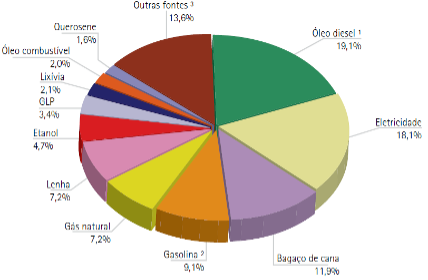
\includegraphics[width=.75\textwidth]{graf-exemplo}	
	\caption*{Fonte: \cite{epe:ben2011}.}
\end{grafico}

As tabelas e os quadros, apesar de possuírem certa semelhança entre si, diferenciam-se não apenas no formato exigido, mas também pelo conteúdo que exibem:

\begin{enumerate}[label=\alph*)]
	\item um quadro apresenta informações ou resultados qualitativos, ou seja, em forma de texto, mesmo que este empregue números;
	\item uma tabela apresenta informações ou resultados quantitativos, ou seja, números tratados estatisticamente.
\end{enumerate}

Quanto ao formato e à apresentação de tabelas e quadros, como se verifica na Tabela~\ref{tbl-exemplo} e no Quadro~\ref{qdr-exemplo}, devem-se observar as seguintes regras~\citep{fibge:nat1993}:

\begin{enumerate}[label=\alph*)]
	\item a moldura das tabelas não deve ser fechada com traços verticais à esquerda e à direita;
	\item deve-se evitar o uso de traços verticais para separar as colunas e de traços horizontais para separar as linhas de uma tabela;
	\item o quadro é um elemento fechado, portanto, deve conter traços horizontais e verticais para separar suas linhas e colunas, além de traços horizontais e verticais para delimitar sua moldura.
\end{enumerate}

\begin{table}[h]
	\centering
	\caption{Exemplo de formatação de uma tabela para a apresentação de resultados}
	\label{tbl-exemplo}
	\begin{tabular}{ccc}
		\hline
		\textbf{Grupos de idade [meses]} & \textbf{Número de indivíduos no grupo} & \textbf{Indivíduos viáveis [\%]} \\
		\hline
		0 -- 10		& 20	& 9,0
\\
		10 -- 15	& 20	& 10,0
\\
		15 -- 20	& 25	& 4,0
\\
		Acima de 20	& 15	& 3,4
\\
		\hline	
	\end{tabular}
	\caption*{Fonte: Produção do próprio autor.}
\end{table}

\begin{quadro}[h]
	\centering
	\caption{Dimensionamento dos elementos de um conversor \textit{boost}}
	\label{qdr-exemplo}
	\begin{tabular}{|p{60mm}|p{60mm}|}
		\hline
		\rowcolor{gray!25}
		\centering \textbf{Elemento ou Grandeza} &  \centering \textbf{Valor ou Modelo}
		\tabularnewline
		\hline
		Tensão de entrada 		& $48 V$
		\\\hline
		Tensão de saída 		& $200 V$
		\\\hline
		Potência de saída 		& $200 W$
		\\\hline
		Frequência de comutação	& $50 kHz$
		\\\hline
		Indutor de entrada 		& $880 \mu H$
	\\\hline
		Capacitor de saída 		& $22 \mu F$
	\\\hline
		Diodo					& $FES8HT$
		\\\hline
		Interruptor				& $IRFP360$	
	\\\hline
	\end{tabular}
	\caption*{Fonte: \cite{menegaz:thesis2005}.}
\end{quadro}

Outros elementos textuais que podem fazer parte do subprojeto de pesquisa são as equações e fórmulas. Para facilitar a leitura, a NBR 15287:2011 exige que as equações sejam destacadas do texto e numeradas com algarismos arábicos entre parênteses, alinhados à margem direita da página, como mostra a Equação~\eqref{eqn-exemplo}. Assim como no caso de figuras, tabelas e quadros, a citação, ou a chamada, de todas as equações ou fórmulas no texto é obrigatória, e sua localização deve acontecer o mais próximo possível do trecho onde são mencionadas pela primeira vez.

\begin{equation}
	\label{eqn-exemplo}
	v_{r}(t) = R \times i(t)
\end{equation}



%%%%%%%%%%%%%%%%%%%%%%%%%%%%%
\section{Conclusões}
\label{sec-conclusoes}

Esta seção é a parte final do Relatório de Pesquisa onde são apresentadas conclusões correspondentes aos objetivos e/ou às hipóteses do trabalho, explicitando a resposta à pergunta do problema de investigação e as possíveis limitações da pesquisa realizada. Deve ainda conter:

\begin{itemize}
	\item Uma compilação dos resultados dos resultados da pesquisa feita;
	\item Quais as principais dificuldades e limitações encontradas durante o estudo; 
	\item As contribuições que o estudo proporcionou nos âmbitos acadêmico, profissional e da sociedade;
	\item Se seus experimentos ou análises falharam, quais as sugestões para corrigir o problema;
	\item Quais as perspectivas ou sugestões de continuidade do trabalho.
\end{itemize}

Opcionalmente, conforme as especificidades de cada Grande Área do Conhecimento, o autor pode utilizar a Seção~\ref{sec-resultados} para apenas apresentação de resultados, deixando a Seção~\ref{sec-conclusoes} para a discussão dos resultados e as conclusões. Neste caso, o título da Seção~\ref{sec-resultados} deverá ser ``Resultados'' e da Seção~\ref{sec-conclusoes}, ``Discussão e Conclusões''.

Por fim, cabe ainda ressaltar que o Relatório Final é individual e deve ser escrito pelo discente bolsista/voluntário de iniciação científica, sob a supervisão/orientação do seu professor orientador. O relatório deverá ser enviado pelo orientador utilizando o Sistema Acadêmico de Pesquisa e Pós-Graduação (SAPPG), a partir do dia de início de envio até a data limite estabelecidos no Edital. O envio do Relatório Final após a data limite fixada implicará nas sanções previstas ao orientador e seu orientando, conforme estabelecido em Edital e no Regulamento Geral do PIIC/UFES, disponível no site da Pró-Reitoria de Pesquisa e Pós-Graduação (PRPPG).




%%%%%%%%%%%%%%%%%%%%%%%%%%%%%
\section*{Agradecimentos}

Esta é uma seção opcional e deve ser utilizada para registrar os agradecimentos do autor do Subprojeto de Iniciação Científica pelo suporte técnico e/ou financeiro recebido de instituições públicas ou privadas. Caso não haja agradecimentos a serem feitos, esta seção deve ser excluída do Relatório Final.


%\bibliographystyle{apalike2}
\bibliographystyle{hapalike2-NOand}

\renewcommand{\bibsection}{\section*{Referências Bibliográficas}}
\bibliography{biblio}


\end{document}



